% Inbuilt themes in beamer
\documentclass{beamer}
\usepackage[UKenglish]{babel}
\usepackage[UKenglish]{isodate}
\cleanlookdateon
\usepackage{siunitx}
\usepackage{amsmath}
\usepackage{amssymb}
\usepackage{gensymb}
\usepackage{float}
\usepackage{lmodern}
\usepackage[T1]{fontenc}
\usepackage[utf8]{inputenc}
%\usepackage[normalem]{ulem}
\usepackage{hyperref}
\hypersetup{
    colorlinks=true,
    linkcolor=blue,
    filecolor=magenta,      
    urlcolor=blue,
    pdfpagemode=FullScreen,
}
\usepackage{lipsum}

\usepackage{graphicx}
\graphicspath{{./images/}}

\usepackage{amsthm}
\setbeamertemplate{theorems}[numbered]
\theoremstyle{definition}
\newtheorem{thm}{Theorem}
\theoremstyle{remark}
\newtheorem{remark}{Remark}

\usepackage{tikz}
\usetikzlibrary{shapes.callouts,tikzmark,calc}
\usepackage{tikzducks}

% Theme choice:
\usetheme{Montpellier}

% Title page details: 
\title{UCL PhySoc {\LaTeX} Workshop}
\author{Neil Booker, Pranav Havalgi Nama}
\date{\today}
%\logo{\large \LaTeX{}}


\begin{document}

% Title page frame
\begin{frame}
\titlepage 
\end{frame}

% Remove logo from the next slides
% \logo{}

\begin{frame}{What we will go through today}
\tableofcontents
\end{frame}

\section{Why {\LaTeX}?}
\begin{frame}{Why {\LaTeX}?}
\begin{figure}[H]
\centering
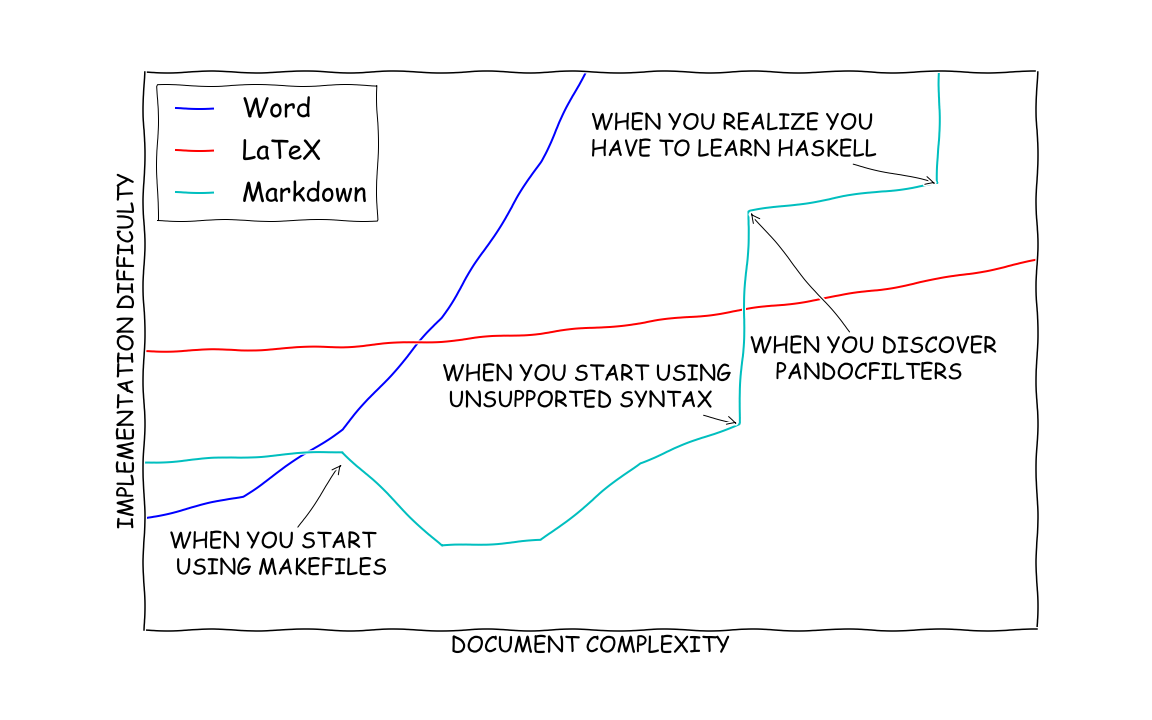
\includegraphics[width=8cm]{Graph.png}
\caption{Oh, \textit{really}?}
\end{figure}
\end{frame}
\begin{frame}{Why it's better than Word!}
\begin{figure}[H]
\centering

\includegraphics[width=11cm]{motivatingmeme.png}
\caption{Eat your heart out, Bill.}
\end{figure}
\end{frame}
\begin{frame}{Fancy motivating examples}
Examples by Senan Sekhon, Khan of Ti\textit{k}Z and {\LaTeX}
\begin{itemize}
\item \href{https://arxiv.org/pdf/2203.14693.pdf}{Supersymmetric Quantum Mechanics}
\item \href{https://www.overleaf.com/latex/examples/periodic-pool-table/cnfychgzwxjk.pdf}{Periodic pool table}
\end{itemize}
\end{frame}


\section{Compilers \& editors}
\begin{frame}{Commonly used editors}
...and a little demo to go with it.
\begin{itemize}
\item TeXworks
\item Overleaf
\item TeXstudio/TeXmaker
\end{itemize}
\end{frame}
\begin{frame}{Pros and cons of commonly used editors}
\begin{itemize}
\item TeXworks 
\begin{itemize}
\item Pros: Comes with MikTeX, simple, very lightweight
\item Cons: Very basic, sometimes needs extra work with bib
\end{itemize}
\item Overleaf
\begin{itemize}
\item Pros: Online (no install), allows collaborators
\item Cons: No extra packages (?), costs, online, closed-source
\end{itemize}
\item TeXstudio/TeXmaker
\begin{itemize}
\item Pros: Way more functionality, spellchecker, autocomplete, symbols libraries\footnotemark\footnotetext{If you call a package-specific symbol, it auto-adds the package on the top of the document.}
\item Cons: Slightly larger size, sometimes slow to run, overwhelming at start
\end{itemize}
\end{itemize}
\end{frame}


\section{Frequently used packages}
\begin{frame}{A list of such packages}
\begin{itemize}
\item \textbf{Encoding packages, largely uninteresting}: fontenc, inputenc, lmodern
\item \textbf{Trivial packages}: amsmath, amssymb/gensymb, physics, graphicx
\item \textbf{Hidden gems}: siunitx, hyperref (custom link colours), float (force image placement), longtable, tabularx, listings (for programmers)
\item \textbf{Ultra-sophisticated stuff}: amsthm/ntheorem, Ti\textit{k}Z (and family), mdframed/tcolorbox
\end{itemize}
\end{frame}


\section{Case studies}

\begin{frame}[fragile]{Now that wasn't so hard, was it?}
\begin{figure}[H]
\centering
{\scriptsize
\begin{verbatim}
                                     You keeping us on course,
                                       Little buddy?           \

      Yes, Skipper \                       __________________________
                   H                      |   ____     _____
     ___           O                      |  |____|   |_____|
    |\_ --------__,+-_____________________|____________________-------
    \  `===#==__|__/\____|_____|_______|_______|_______|_____-------
     \
      |   ss. minnow
       \
    ~~~~-\_ /~~=._         ~~~~~~~~~~~             ~~~~~~~~~~~~~
~~~~      =/       ~~~~~~~~ ~~~~~~    ~~~~~~~~~~~~~             ~~~~~
\end{verbatim}}
\caption{\href{https://www.youtube.com/watch?v=b4qRp4OfUn8&t=263s}{Famous last words in {\LaTeX}}}
\end{figure}
\end{frame}
\begin{frame}{Equation basics}
$$\frac{d}{d\lambda}\left(\frac{\partial L}{\partial\dot{q}}\right)=\frac{\partial L}{\partial q}$$
$$\delta^a_b=\begin{cases}1&a=b\\0&a\ne b\end{cases}$$
$$ds^2=-dt^2+dx^2+dy^2+dz^2\leftrightarrow g_{ij}=\begin{pmatrix}-1&&&\\&1&&\\&&1&\\&&&1\end{pmatrix}$$
\end{frame}
\begin{frame}{Environments}
$$
\begin{aligned}
R_{t t}&=e^{\nu-\lambda}\left[\frac{1}{2} \nu''+\frac{1}{4}\left(\nu'\right)^2+\frac{1}{r} \nu'-\frac{1}{4} \nu' \lambda'\right]\\
R_{r r}&=-\frac{1}{2} \nu''-\frac{1}{4}\left(\nu'\right)^2+\frac{1}{4} \nu' \lambda'+\frac{1}{r} \lambda' \\
R_{\theta \theta}&=1-e^{-\lambda}+\frac{1}{2} r \lambda' e^{-\lambda}-\frac{1}{2} r \nu' e^{-\lambda} \\
R_{\phi \phi}&=\sin ^2 \theta R_{\theta \theta}
\end{aligned}
$$
\begin{center}
\begin{tabular}{|c|c|c|} 
\hline
Property & Natural unit & Conversion to SI\\\hline
Energy & GeV & Multiply by constants\\\hline
Momentum & GeV/c & Reinsert $c$ and multiply by constants\\\hline
\end{tabular}
\end{center}
Here is some text\footnotemark\footnotetext{And here is a footnote.}. Here is a \href{https://www.youtube.com/watch?v=dQw4w9WgXcQ}{hyperlink} and an \href{mailto:example@example.org}{e-mail address}.
\end{frame}
\begin{frame}{Image placement}
\begin{figure}[H]
\centering

\includegraphics[width=5cm]{Dramatic_Chipmunk.png}
\caption{The image, when you place it without the \textit{float} package.}
\end{figure}
\end{frame}
\begin{frame}{Blocks in beamer}
\begin{block}{Standard block}
This is a standard block.
\end{block}
\begin{alertblock}{Alert block}
This block presents an alert message.
\end{alertblock}
\begin{exampleblock}{Example block}
Warning: examples not included.
\end{exampleblock}
\end{frame}
\begin{frame}[fragile]{Theorems}
\begin{thm}[\textit{The Big Lebowski}]
When you start working with {\LaTeX}, you're entering a world of pain.
\end{thm}
\begin{remark}
This is a shitty theorem. More sophisticated theorems can be implemented with Ti\textit{k}Z, often outside Beamer:
\end{remark}
\begin{verbatim}
\usepackage{tikz}
\usepackage{mdframed}
\usepackage{ntheorem}
\theorembodyfont{\upshape}
\mdfdefinestyle{default}{hidealllines=true, topline=true, 
linewidth=5pt, leftmargin=2, rightmargin=2}
\newmdtheoremenv[style=default, backgroundcolor=blue!10, 
linecolor=blue]{definition}{Definition}[section]
\end{verbatim}
\end{frame}

\begin{frame}{Lipsum (oh wait... wrong one)}
What the fuck did you just fucking say about me, you little bitch? I'll have you know I graduated top of my class in the Navy Seals, and I've been involved in numerous secret raids on Al-Quaeda, and I have over 300 confirmed kills. I am trained in gorilla warfare and I'm the top sniper in the entire US armed forces. You are nothing to me but just another target. I will wipe you the fuck out with precision the likes of which has never been seen before on this Earth, mark my fucking words. You think you can get away with saying that shit to me over the Internet? Think again, fucker. As we speak I am contacting my secret network of spies across the USA and your IP is being traced right now so you better prepare for the storm, maggot. The storm that wipes out the pathetic little thing you call your life. You're fucking dead, kid. I can be anywhere, anytime, and I can kill you in over seven hundred ways, and that's just with my bare hands. Not only am I extensively trained in unarmed combat, but I have access to the entire arsenal of the United States Marine Corps and I will use it to its full extent to wipe your miserable ass off the face of the continent, you little shit. If only you could have known what unholy retribution your little "clever" comment was about to bring down upon you, maybe you would have held your fucking tongue. But you couldn't, you didn't, and now you're paying the price, you goddamn idiot. I will shit fury all over you and you will drown in it. You're fucking dead, kiddo.
\end{frame}

\begin{frame}{Lipsum (take 2)}
\lipsum
\end{frame}

\begin{frame}{Beginnings of Ti\textit{k}Z}
\begin{figure}[H]
\centering

\begin{tikzpicture}[scale=1]
\duck[bubblecolour=white!95!yellow, eye=green, bill=black, devil=black, body=red, scale=2];
\node[rectangle callout, draw, text width=4.5cm, align=center, xshift=-2cm, yshift=4.5cm, callout absolute pointer={(bill)}, callout pointer shorten=0.5cm] {I am an evil Ti\textit{k}Zduck and I am plotting your demise in the end-of-year exams};
\end{tikzpicture}
\caption{An evil Ti\textit{k}Zduck plots your demise in the end-of-year exams}
\end{figure}
\end{frame}

\begin{frame}{Examples Q\&A session}
Ask yer questions before it's too late!
\end{frame}

\section{General Q\&A session}
\begin{frame}{General Q\&A session}
No, really.
\end{frame}

\section{Conclusion}
\begin{frame}{Conclusion}
\begin{figure}[H]
\centering

\includegraphics[width=6.5cm]{ctanerror.png}
\end{figure}
\end{frame}

\section{Further reading}
\begin{frame}{Further reading}
\begin{itemize}
\item \href{https://www3.nd.edu/~nmark/UsefulFacts/LaTeX_symbols.pdf}{The Great, Big List of {\LaTeX} Symbols}
\item \href{https://cremeronline.com/LaTeX/minimaltikz.pdf}{A very minimal introduction to Ti\textit{k}Z}
\item \href{https://mirror.apps.cam.ac.uk/pub/tex-archive/graphics/pgf/base/doc/pgfmanual.pdf}{Ti\textit{k}Z \& PGF Manual} (advanced)
\end{itemize}
\end{frame}
\end{document}